\icode{E-MM-MU-L3-261014-001}
如图所示，在足够大的光滑水平地面上，静置一质量为\(2m\)的滑块，滑块右侧面的\(\sfrac{1}{4}\)光滑圆弧形槽的半径为\(R\)，末端切线水平，圆弧形槽末端离地面的距离为\(\sfrac{R}{4}\)。质量为\(m\)的小球(可视为质点)从圆弧形槽顶端由静止释放，与滑块分离后做平抛运动，重力加速度大小为\(g\)，下列说法正确的是\paren[]

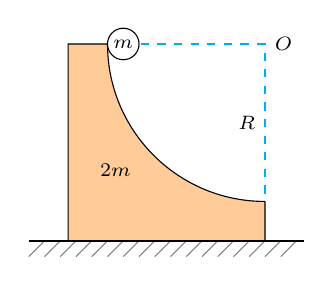
\begin{tikzpicture}[font=\scriptsize]
	\draw[fill=orange!40] (0,0) arc(-90:-180:2)--(-2.5,2)--(-2.5,-.5)--(0,-.5)--(0,0);
	\draw[dashed,cyan] (-2,2)--(0,2)node[right,black]{\(O\)}--node[left,black]{\(R\)}(0,0);
	\draw[fill=white] (-1.8,2)node{\(m\)} circle(.2);
	\foreach \x in {-3,-2.8,...,.3}
		\draw[gray] (\x,-.7)--++(.2,.2);
	\draw[thick] (-3,-.5)--(.5,-.5);
	\node at(-1.9,.4){\(2m\)};
\end{tikzpicture}
\begin{choices}
	\item 滑块的最大动能为\(\frac{mgR}{3}\)
	\item 小球离开滑块时的动能为\(\frac{11mgR}{12}\)
	\item 小球落地时的动能为\(mgR\)
	\item 小球落地时与圆弧形槽末端抛出点的距离为\(\frac{5R}{4}\)
\end{choices}
\begin{answer}
   AD\qquad 提示：滑到圆弧末端时，\(v_1 = 2 \sqrt{\frac{gR}{3}}\) \quad \(v_2 = \sqrt{\frac{gR}{3}}\)
\end{answer}